\chapter{\label{chap:evaluation}Evaluation}

% - trust explorer example
% - 9 fully functional modules
% - demonstrate the viability of run-time changes and alternative algorithmic approaches
% - open questions:
%   - how do we evaluate this?
%   - how do we show that it works as intended?
%   - we successfully bypassed the Android security model with protection against dynamic code injection using Webview
%   - pure technical (module loading times, memory usage impact, event-driven impact, event processing workload analysis, peak performance estimation)
%   - Github/NodeJS/Debian replacement workload analysis ("github is the largest code host in the world, with 20 million users and more than 57 million repositories"

This chapter will evaluate the proposed framework, FBase, described in Section~\ref{chap:design}. The evaluation consists of two parts, which will show if FBase, satisfies the requirements determined in Chapter~\ref{chap:requirements}:\newline

\begin{itemize}[nosep]
	\item Testing if the concept works and is viable.
	\item Examining the effectiveness of the discovery protocol% and the module communication.
\end{itemize}

\section{Testing the Viability of the Concept}

To determine if the concept works and is viable, this thesis uses one non-trivial use-case. This use-case comes from a project called Tribler.

\subsection{Tribler}

Tribler is an open-source community-driven decentralized BitTorrent client being developed and researched at the Delft University of Technology. Its main feature is that it allows anonymous peer-to-peer communication by default. It is built on the underlying network library IPv8, also being worked on by the same group.

Besides handling the tasks of a standard BitTorrent client, Tribler also makes it possible to:

\begin{itemize}
	\item \textbf{Search for content: } allowing the program to operate independently of external content search providers that could be blocked and made it immune to limiting external actions such as legal constraints. Which is happening more frequently nowadays.
	\item \textbf{Torrent anonymously: } routing torrent traffic through anonymized tunnels that operate using the same principle as the TOR stack. Providing pseudo-anonymity for the two end and other observing parties.
	\item \textbf{Accumulate trust: } all torrenting metadata is stored in a way that is not linked to an physical identity or an IP address. This data is then translated into a trust score by calculating the ratio between the amount of traffic communicated across the network. A positive seed ratio (the ratio between uploading content and downloading content) indicated a positive trust value.
	\item \textbf{Trade trust: } With this trust system it is possible to prioritize or refuse services for particular users. To increase the incentive for having a large seeder network and therefore a high trust value, Tribler allows users with a large amount of uploaded content to exchange this gathered trust for currency on the built-in marketplace inside the Tribler application.
\end{itemize}

This trust value, expressed as reputation inside the Tribler application, can be described as an up- and download currency in a reputation-based peer-to-peer network. When a peer uploads more than it downloads, the reputation of that peer increases, and the peer can download more effectively.

\subsection{Trust Experiment}

The experiment consists of conducting a use-case study, by creating a fully functioning example that demonstrates the composition and construction of an application with interchangeable trust models. This application will consist of 6 components:

\begin{itemize}
	\item Test application GUI (view layer)
	\item Test application (logic layer)
	\item Trust algorithm 1 (logic layer)
	\item Trust algorithm 2 (logic layer)
	\item Execution engine (infrastructure layer)
	\item Transport engine (infrastructure layer)
\end{itemize}

%Figure~\ref{fig:experiment} shows an overview of the example application.
The domain of trust was chosen since this is a very interesting use-case that has not been explored yet in other works. It allows users of a system to define their own notion of the concept of trust and apply this to their system without requiring extensive knowledge about each application they are using. For this experiment, this work makes use of two different trust algorithms: Netflow and PimRank. These two algorithms act as an example for this experiment.

%\begin{figure}[h]
%	\centering
%	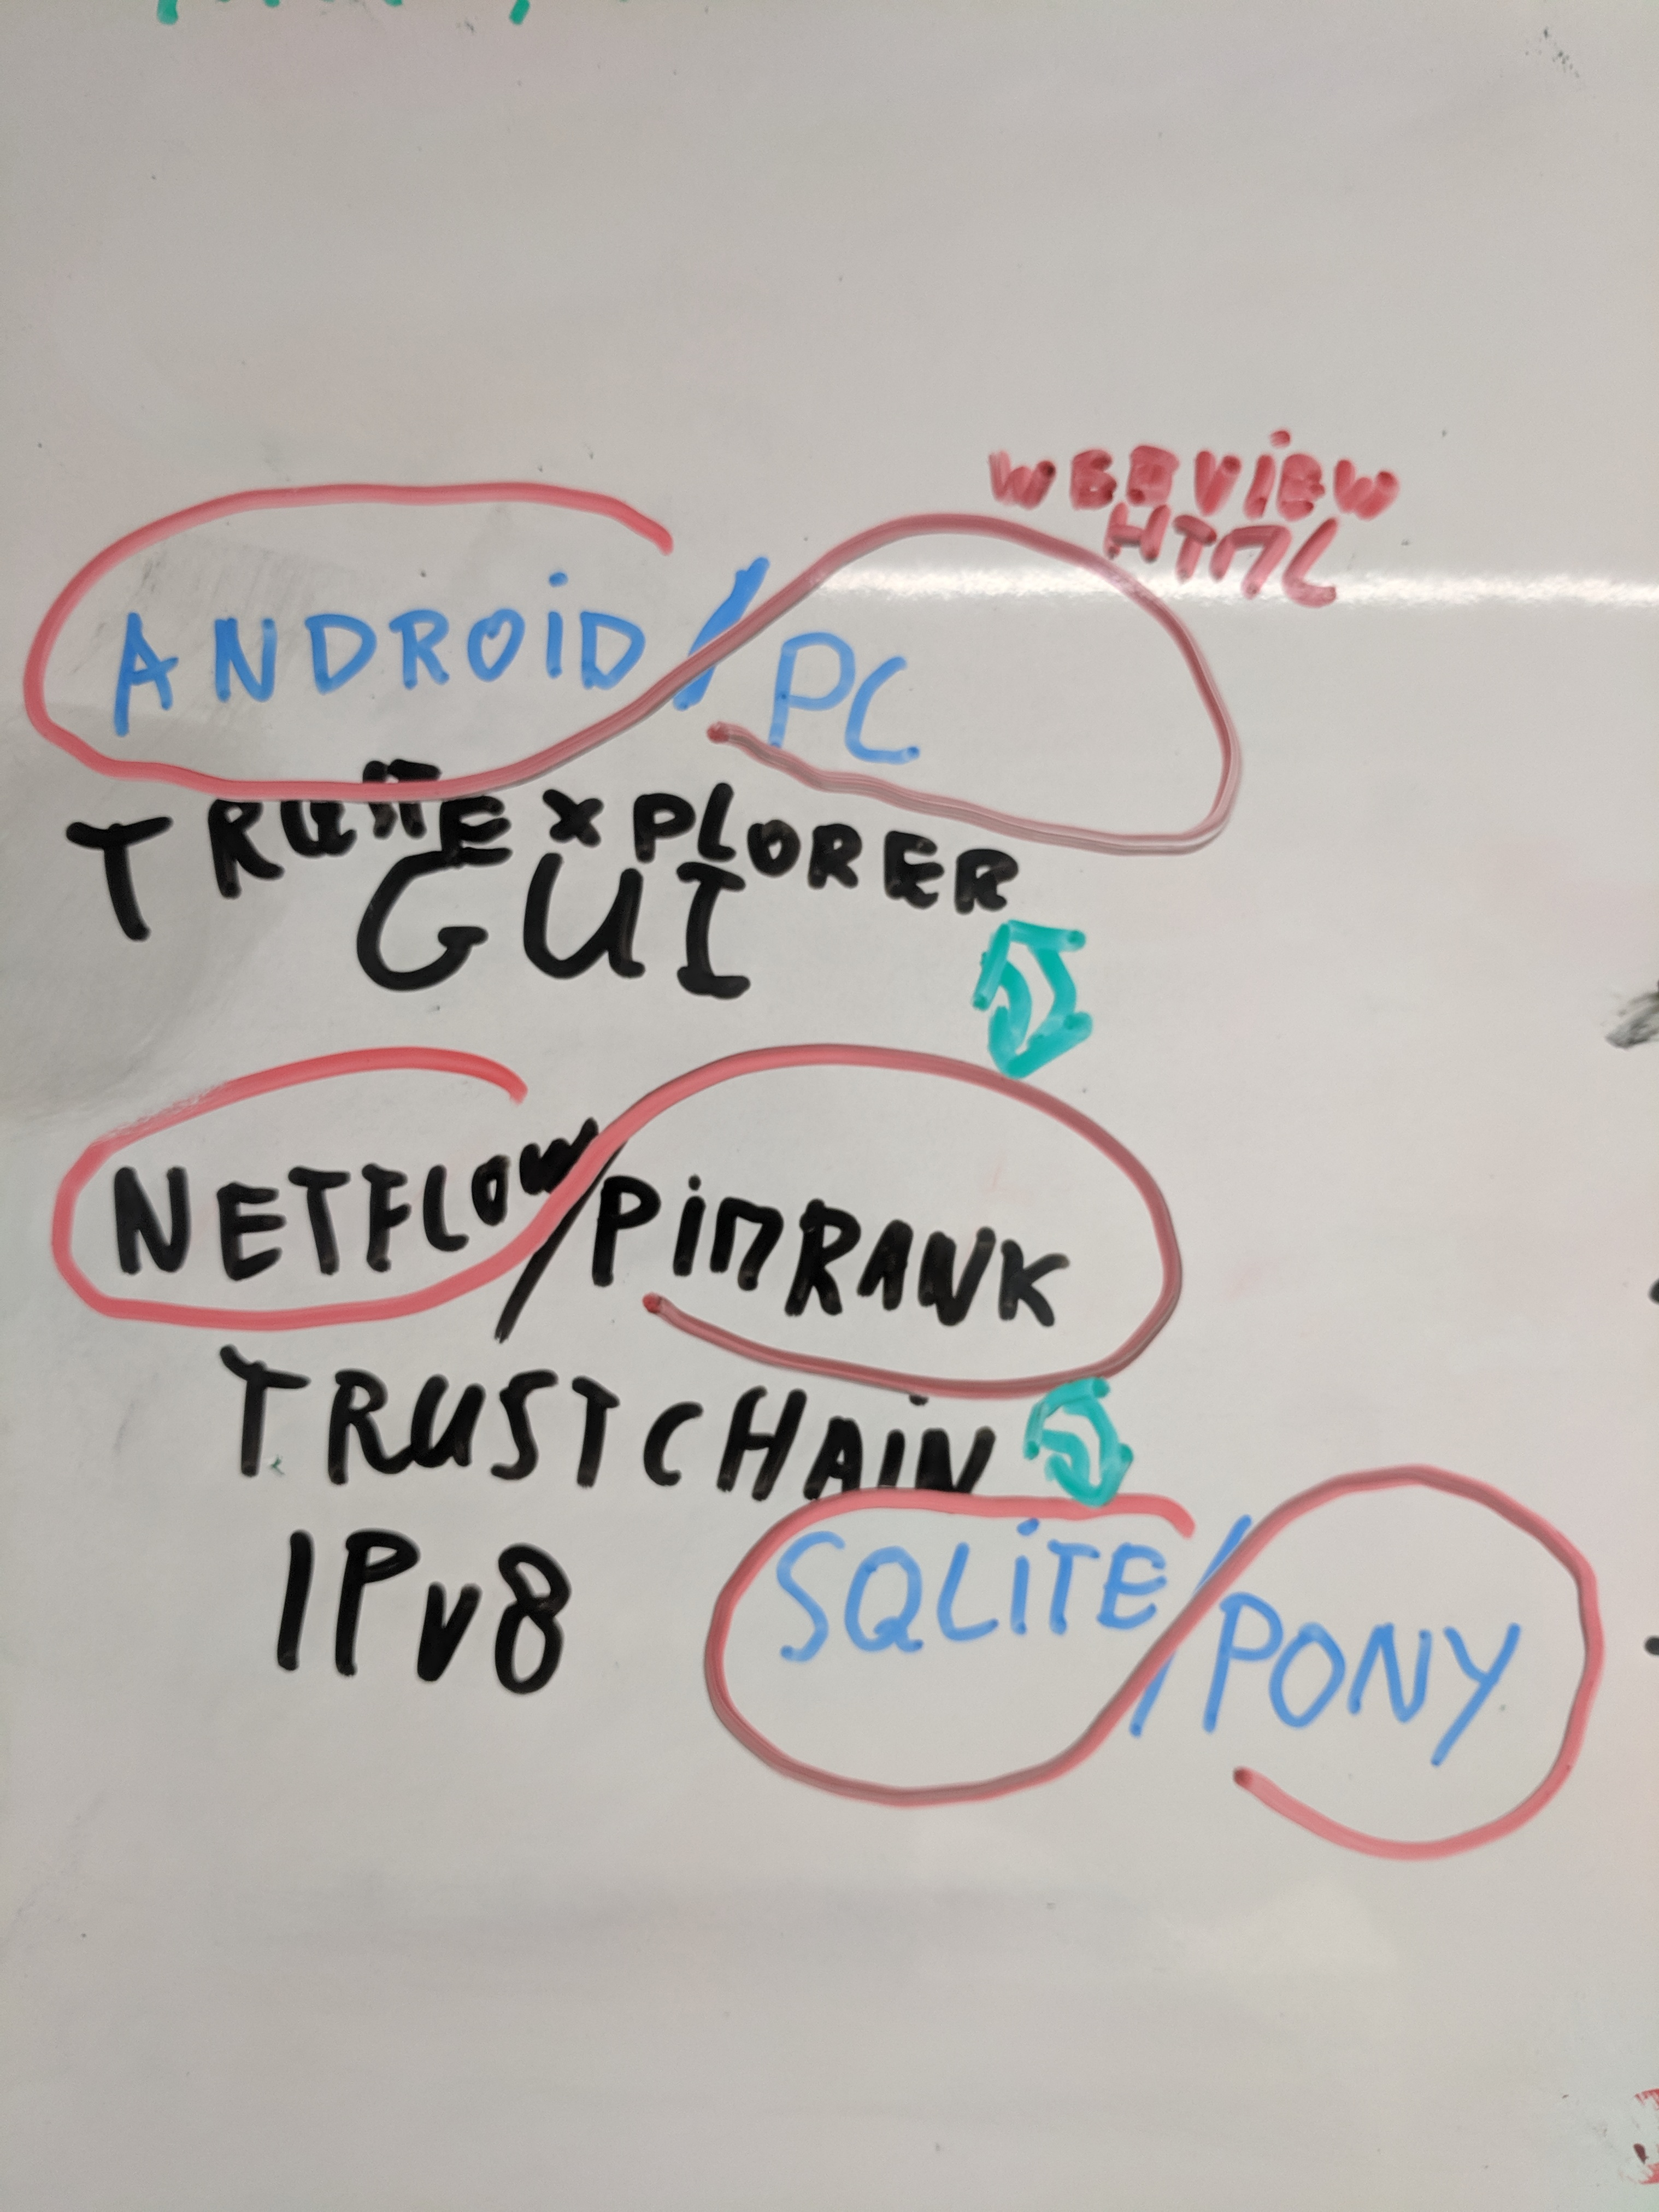
\includegraphics[width=0.5\textwidth]{images/experiment.jpg}
%	\caption{\label{fig:experiment} Trust experiment use-case}
%\end{figure}

\subsection{Mobile App Experiment}

To test the robustness and flexibility of the framework, an experiment was performed to try to create a proof-of-concept prototype of an Android application that could run the same stack of code to extend the ecosystem to mobile platforms. Since the two major mobile platforms (Android, iOS) only run applications custom made for these platforms, different methods had to be explored. Because iOS has a very restricted development environment and strict security policies, this route was not further explored.

The Android platform allows app developers to run Java, Kotlin (Java-based), and C. The desired framework language (Python) does not natively run on this platform. Converting the project code and dependencies is not a simple or maintainable method. This approach, however, also would not work. To improve security, the Android platform makes use of app scanning to verify that the executables haven't been tampered with. This security method severely hinders the working of the framework, since more functionality is added by the distribution of applications through its peer-to-peer network. These new code inclusions would trigger warnings in the Android security system and would block the app.

To circumvent this, a un-official method was used to package all the necessary code, dependencies, and executables as a single file and execute this as a C service on the Android platform. To accomplish this, a project called Python-for-Android was used. Python-for-Android is a build script that compiles the desired Python system version and Python dependencies for the ARM platform and creates a directory structure that can be used to run on Android. In Figure~\ref{fig:android-architecture} and overview of the Android app structure can be seen.

\begin{figure}[h!]
	\centering
	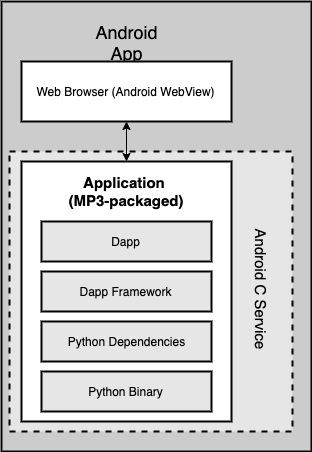
\includegraphics[width=0.5\textwidth]{images/android-app.png}
	\caption{\label{fig:android-architecture} Android app architecture.}
\end{figure}

Since the Android app is needed to interact with the C service in the background, a part of the app had to be written in either Java or Kotlin. To keep this amount of code to a minimum, a decision was made to create all GUIs in web technologies, so the view layer can be shared between mobile and desktop platforms. This decision made it possible to include a web browser as the only component written for the mobile platform. This web browser can then interact with the webserver and REST API running on the C service.

To package the executable code in a way that would not trigger the Android security system, the code had to be bundled in a single file, disguised as an MP3. This format does not get checked by the Android security system and therefore can be used for this work. Underneath the extension, the code is packaged as a GZIP Tar-archive. Upon running the Android application, this MP3 file is unpacked in the application space of the app and the C service is started with the right configuration to run the code.

%In Figure~\ref{fig:android-app} a screenshot can be seen of the framework running with a test dApp on the Android platform. 

Development was stopped after reaching the proof-of-concept stage as it is not the main goal of this work and the development cycle is very tedious and slow. Each time a change or addition is made to the Framework the entire app structure has to be rebuild. This process can take up to 20 minutes. 

%\begin{figure}[h!]
%    \centering
%    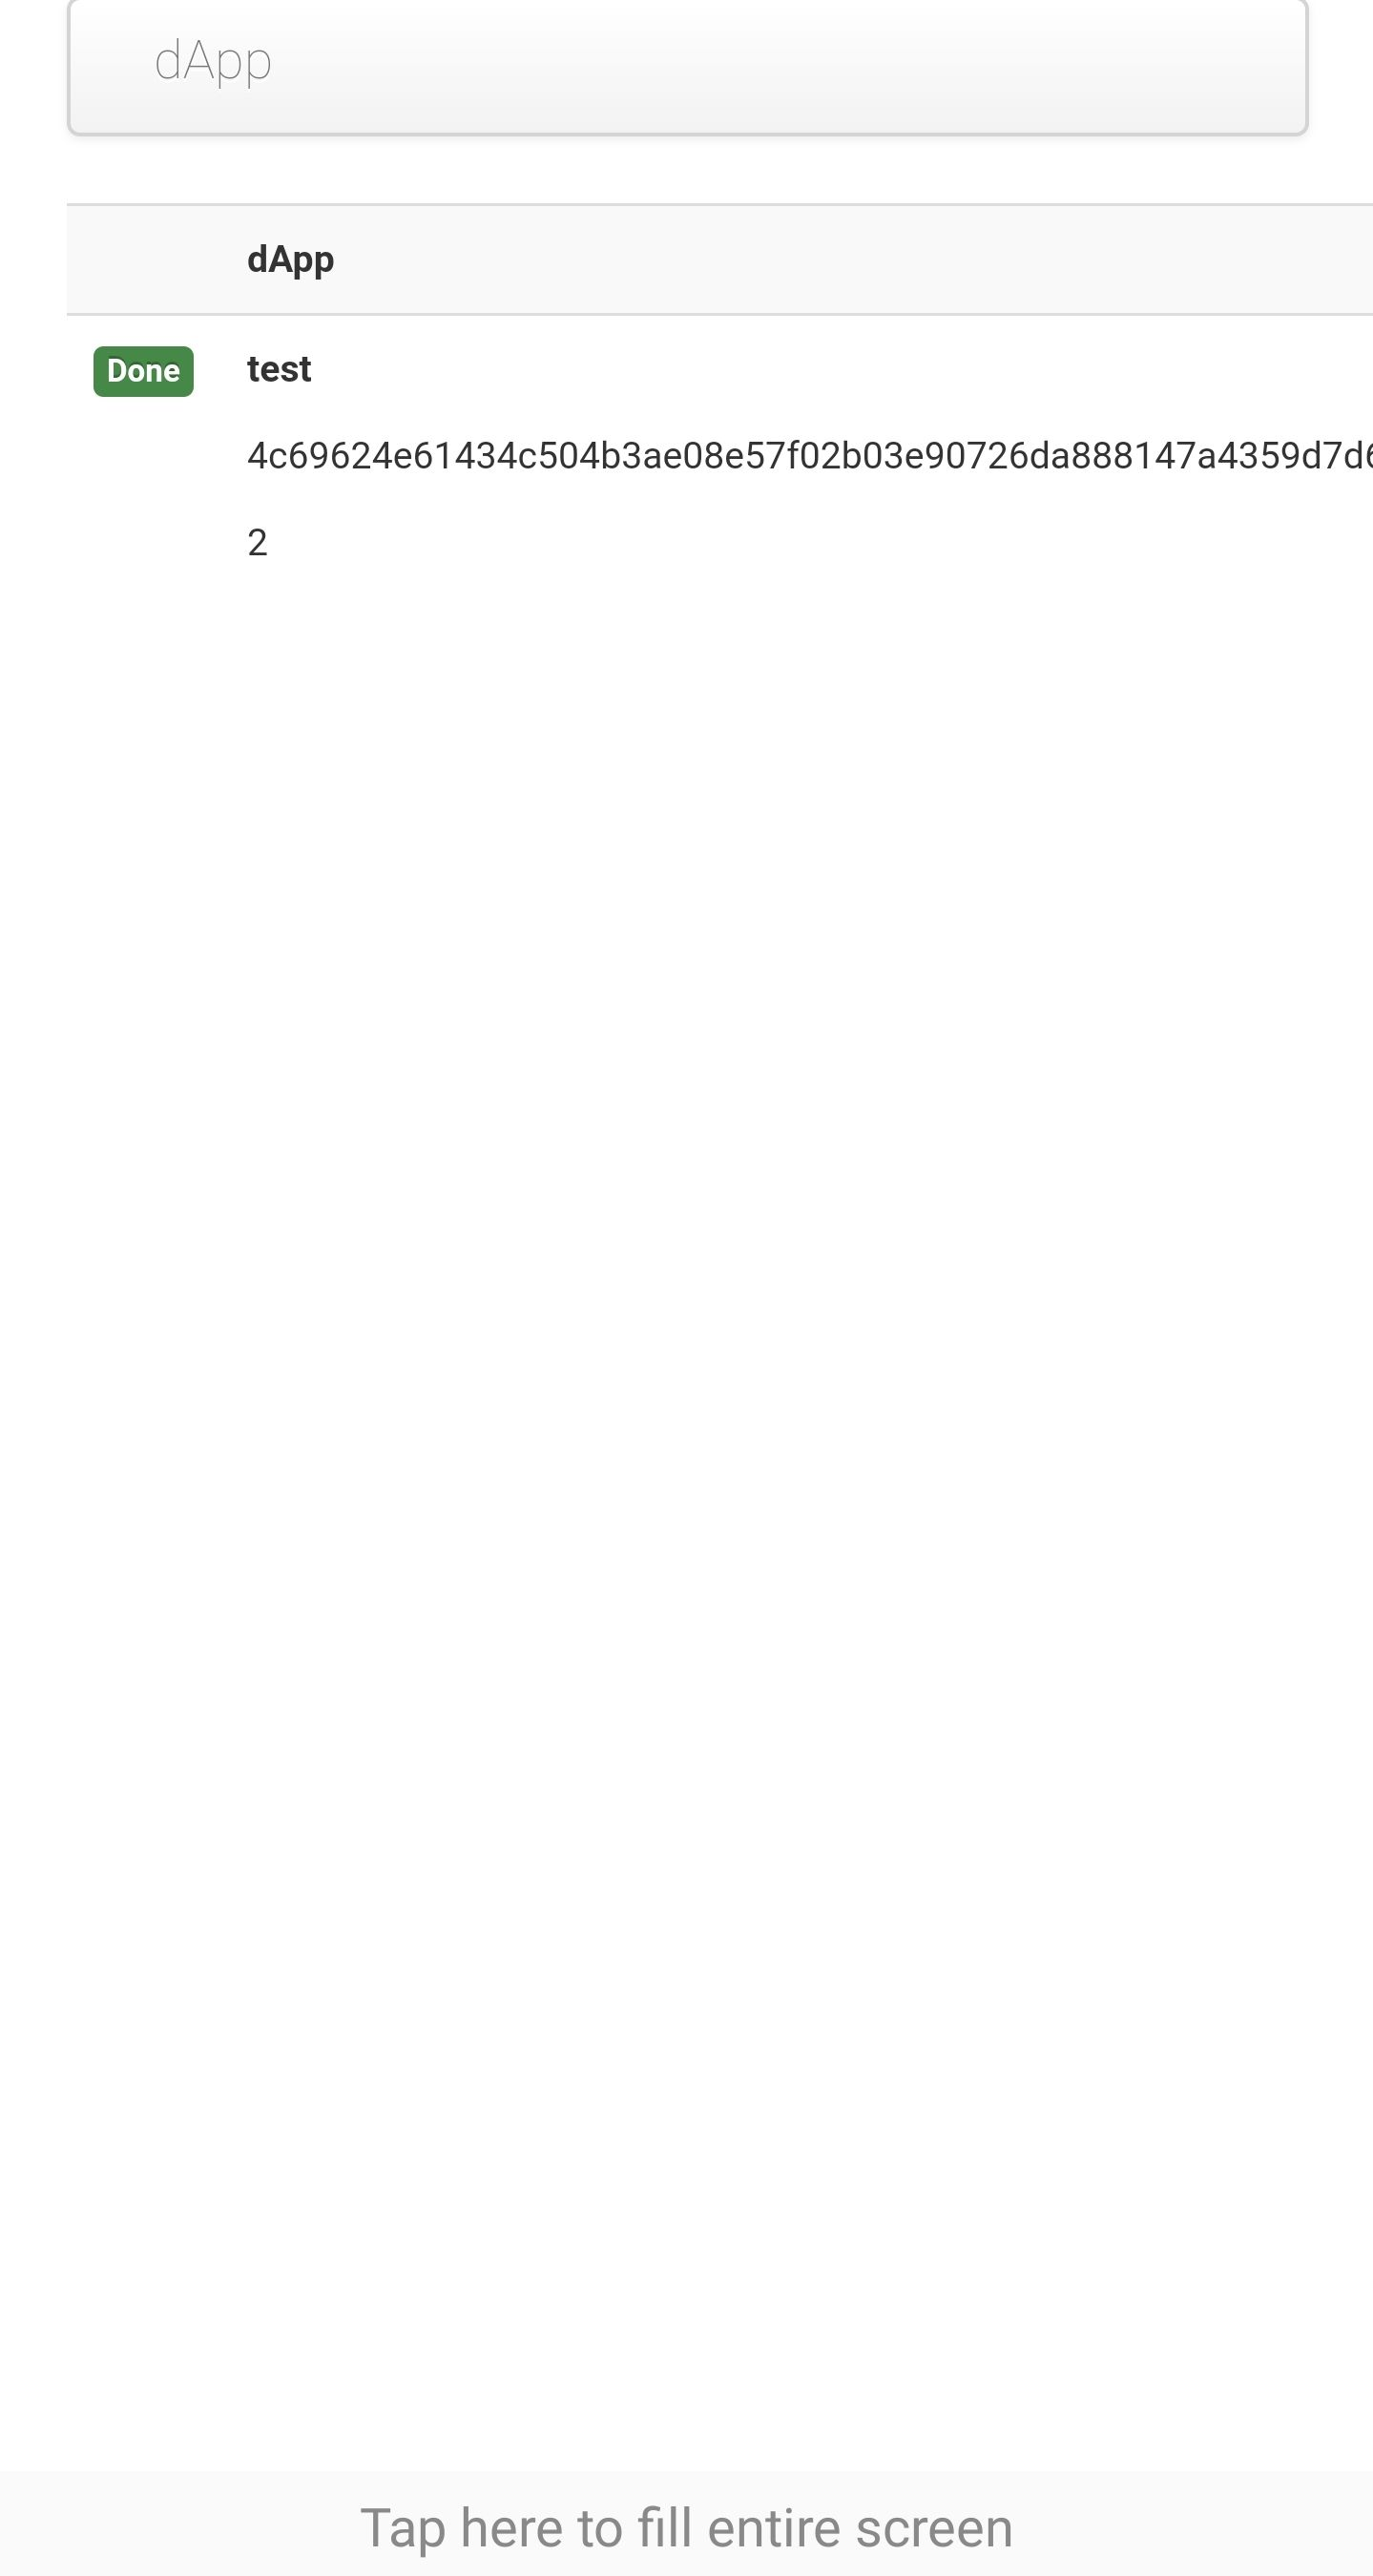
\includegraphics[width=0.5\textwidth]{images/android-app-screenshot.jpg}
%    \caption{\label{fig:android-app}}
%\end{figure}

\subsection{Result Interpretation}

One part of evaluating FBase is testing if the concept works and is viable. Through the use of a non-trivial use-case, it was demonstrated that real-world practical problems can be solved using this framework.

The main advantage that the framework provided in the use-case was the introduction of modularity. On one hand, it has the benefit of flexibility and variety in use. On the other hand, modularization improves the manageability of maintenance for complex software like Tribler.

One of the disadvantages that followed from the use-case was the increased time that modules on FBase took to develop the application compared to implementing it in a monolithic architecture. A second more general disadvantage is that the module interconnect limits the complexity of the interaction between modules. This disadvantage did not limit the development of this use-case but changes the way applications need to be developed.

%allows complex software to be manageable for the purpose of maintenance

\section{Effectiveness of the Discovery Protocol}

%\subsection{Sensitivity Analysis}

One of the most important components of FBase is the module discovery protocol. To make this platform usable, this mechanism has to perform sufficiently effective without crippling the network with its overhead. The discovery protocol is compared to existing methods and the effectiveness is evaluated based on a theoretical sensitivity analysis.

\subsection{Existing Methods}

One of the simplest and easiest approaches that can be taken to discover new modules is flooding information packets throughout the network. This is the fastest approach for discovering modules, however, it will create a big strain on the network when then network becomes larger. It also allows malicious nodes to DDOS the network with relative ease.

Another approach is crawling. When crawling, nodes ask their neighboring nodes for the modules they have discovered. This approach is much less intensive on the global network as it works on a localized view. This method will eventually create a global coverage for module discovery, however, this method is very slow. Each module has to be propagated through each local view. This method is not suitable for large scale module discovery.

\subsection{Sensitivity Analysis}

FBase makes use of a discovery protocol based on a voting mechanism to prevent DDOSing while still being able to effectively discover new modules. It uses selective flooding on a local scale. Flooding is a effective way to reach a large number of nodes connected in a graph as can been seen in Figure~\ref{fig:discovery-flooding}. Even when there is a significant overlap in the neighbors of the nodes, thousands of nodes can be reached in very few steps.

\begin{figure}[ht!]
	\centering
	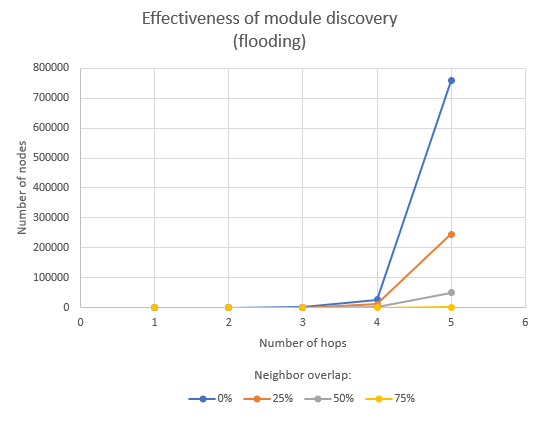
\includegraphics[width=0.64\textwidth]{images/discovery-flooding.png}
	\caption{\label{fig:discovery-flooding} Effectiveness of module discovery (flooding).}
\end{figure}
%\begin{table}[h!]
%    \begin{tabular}{l|lllll}
%        \toprule
%        Neighbor overlap & 1     & 2      & 3        & 4           & 5              \\ \midrule
%        0\%              & 1 (0) & 31 (1) & 901 (31) & 26131 (901) & 757801 (26131) \\
%        25\%             & 1 (0) & 24 (1) & 530 (24) & 11662 (530) & 244904 (11662) \\
%        50\%             & 1 (0) & 16 (1) & 241 (16) & 3375 (241)  & 50385 (3375)   \\
%        75\%             & 1 (0)                      & 9 (1)  & 65 (9)   & 392 (65)    & 2289 (392) \\ \bottomrule   
%    \end{tabular}
%\end{table}

\newpage

However, If the same analysis is run with the voting mechanism the results are not as effective. The reason behind this behavior is that only a small fraction of all users will vote on a specific module. For this analysis, this percentage is set at 1\% of all nodes. Even in the most optimistic scenario where there is no neighbor overlap, the discovery stops after two steps with 24 nodes being aware of the module.

To circumvent this problem FBase uses the concept of Seed Discovery where multiple seed points are used for discovery when the author creates a module. This increases the chance for one of these starting points to overcome this barrier. This effect can be seen in Figure~\ref{fig:discovery-fbase-simple-0}. However, when applying Seed Discovery only when a module is created the discovery process still halts after 6 steps with 101 starting points.

\begin{figure}[ht!]
	\centering
	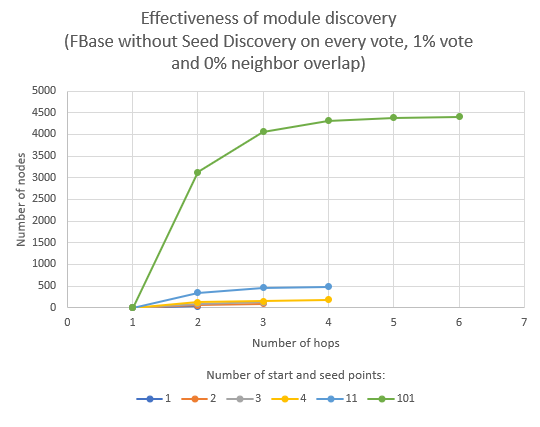
\includegraphics[width=0.64\textwidth]{images/discovery-fbase-simple-0.png}
	\caption{\label{fig:discovery-fbase-simple-0} Effectiveness of module discovery (FBase without Seed Discovery on every vote, 1\% vote and 0\% neighbor overlap)}
\end{figure}

%1\% vote and 100\% disconnected
%\begin{table}[h!]
%    \begin{tabular}{@{}l|llllllll@{}}
%        \toprule
%        S & 1     & 2        & 3         & 4         & 5         & 6         & 7     \\ \midrule
%        1   & 1 (0) & 31 (1)   &     &        &           &           &               \\
%        2   & 1 (0) & 62 (1)   & 91 (2)    &     &      &           &               \\
%        3   & 1 (0) & 93 (1)   & 122 (2)   &    &        &           &               \\
%        4   & 1 (0) & 124 (1)  & 153 (2)   & 182 (3)   &    &       &               \\
%        ... &       &          &           &           &           &           &             \\
%        11  & 1 (0) & 341 (1)  & 457 (4)   & 486 (5)   &    &       &     \\
%         &       &          &           &           &           &           &     \\
%        101 & 1 (0) & 3131 (1) & 4059 (32) & 4320 (41) & 4378 (43) & 4407 (44) &  \\ \bottomrule
%    \end{tabular}
%\end{table}

In a more realistic scenario where there would be a 25\% overlap between the neighbors of nodes, the result would be even less effective as can be seen in Figure~\ref{fig:discovery-fbase-simple-25}.

\begin{figure}[ht!]
	\centering
	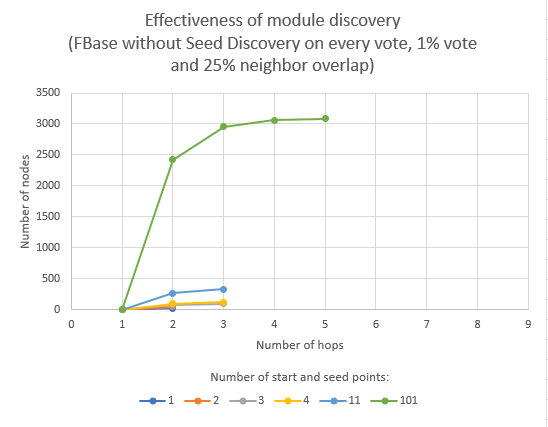
\includegraphics[width=0.64\textwidth]{images/discovery-fbase-simple-25.png}
	\caption{\label{fig:discovery-fbase-simple-25} Effectiveness of module discovery (FBase without Seed Discovery on every vote, 1\% vote and 25\% neighbor overlap)}
\end{figure}

%1\% vote and 25\% disconnected
%\begin{table}[h!]
%    \begin{tabular}{@{}l|llllllll@{}}
%        \toprule
%        S & 1     & 2        & 3         & 4         & 5         & 6         & 7     \\ \midrule
%        1   & 1 (0) & 24 (1)   &     &        &           &           &               \\
%        2   & 1 (0) & 48 (1)   &     &     &      &           &               \\
%        3   & 1 (0) & 72 (1)   & 94 (2)   &    &        &           &               \\
%        4   & 1 (0) & 96 (1)  & 118 (2)   &    &    &       &               \\
%        ... &       &          &           &           &           &           &             \\
%        11  & 1 (0) & 264 (1)  & 330 (4)   &    &   &       &     \\
%        ... &       &          &           &           &           &           &     \\
%        101 & 1 (0) & 2424 (1) & 2952 (25) & 3062 (30) & 3084 (31) &  &  \\ \bottomrule
%    \end{tabular}
%\end{table}

\newpage

When the Seed Discovery is applied on every vote, a continuous discovery can be found with 11 starting points as can be seen in Figure~\ref{fig:discovery-fbase-extended-25}.

\begin{figure}[ht!]
	\centering
	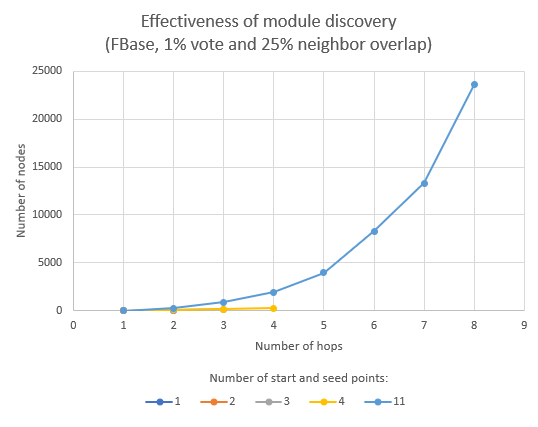
\includegraphics[width=0.64\textwidth]{images/discovery-fbase-extented-25.png}
	\caption{\label{fig:discovery-fbase-extended-25} Effectiveness of module discovery (FBase without Seed Discovery on every vote, 1\% vote and 25\% neighbor overlap)}
\end{figure}

%1\% vote and 25\% disconnected and direct random discovery
%\begin{table}[h!]
%    \begin{tabular}{@{}l|llllllllll@{}}
%        \toprule
%        S & 1     & 2        & 3         & 4         & 5         & 6         & 7   & 8 & 9  \\ \midrule
%        1   & 1 (0) & 24 (1)   &     &        &           &           &      & &         \\
%        2   & 1 (0) & 48 (1)   &    &     &      &           &         & &      \\
%        3   & 1 (0) & 72 (1)   & 142 (2)(1)   &    &        &           &      & &         \\
%        4   & 1 (0) & 96 (1)  & 166 (2)(1)  & 236 (3)(2)   &    &       &     & &          \\
%        ... &       &          &           &           &           &           &      & &       \\
%        11  & 1 (0) & 264 (1)  & 882 (4)(3)   & 1912 (9)(8)  &  3972 (19)(18)  &  8298 (40)(39)     &  13292 (83)(61) &  23592 (133)(111) & ... \\ \bottomrule
%    \end{tabular}
%\end{table}

This approach results in an effective discovery without flooding the network and preventing malicious attempts.

%\section{Requirement Assessment}
%
%To evaluate FBase as a concept, the individual parts that make up the framework need to be evaluated and see if they conform to the requirements set in Chapter 2.
%
%\begin{itemize}[nosep]
%    \item Testing if the concept works and is viable.
%    \item Examining the effectiveness of the discovery protocol% and the module communication.
%\end{itemize}

\subsection{Result Interpretation}

The effectiveness of the discovery protocol is the second part that was analyzed in this evaluation. The sensitivity analysis indicated that a degree of flooding is necessary to accomplish effective network coverage without putting excessive strain on the network. When comparing different situations of selective flooding by introducing voting, it was shown that seed discovery is necessary on every vote for the discovery to reach global coverage.

